%%%%%%%%%%%%%%%%%%%%%%%%%%%%%%%%%%%%%%%%%%%%%%%%%%%
%
%  New template code for TAMU Theses and Dissertations starting Fall 2012.  
%  For more info about this template or the 
%  TAMU LaTeX User's Group, see http://www.howdy.me/.
%
%  Author: Wendy Lynn Turner 
%	 Version 1.0 
%  Last updated 8/5/2012
%
%%%%%%%%%%%%%%%%%%%%%%%%%%%%%%%%%%%%%%%%%%%%%%%%%%%
%%                           SECTION  - Introduction
%%%%%%%%%%%%%%%%%%%%%%%%%%%%%%%%%%%%%%%%%%%%%%%%%%%
\chapter{\uppercase {Introduction}}
\label{sec::Intro}

%%%%%%%%%%%%%%%%%%%%%%%%%%%%%%%%%%%%%%%%%%%%%%%%%%%
%%%   Section - Purpose
\section{Motivation and Purpose of the Dissertation}
\label{sec::Intro_Purpose}

Accurate solutions of the neutral particle transport equation are important for multiple fields, including medical imaging, radiotherapy, nuclear power, and other industrial applications. As computing systems continue to advance, the fidelity of these solutions continues to increase as well. Currently, computational resources on High-Performance Computers (HPC) are at the petaflop level. At this time, there is currently a motivation within the United States Department of Energy (DOE) to one day achieve exascale levels of computing \cite{bergman2008exascale}. However, this move to exascale computing levels will require significantly different computer architectures than what are currently utilized. These changes will include less available memory per process node and will most likely result in a higher frequency of faults or performance fluctuations. Therefore, future parallel algorithms and methods that will make use of exascale computing levels, need to be observant of these architectural changes.

Traditionally, solutions of the neutral particle transport equation have required the use of the most advanced computer hardwares (available at a given time) due to the fidelity required for each dimension of their high-dimensional phase space. This means that further development of transport methods on modern HPCs is beholden to the exascale level limitations. At the exascale level, high-fidelity numerical transport solutions could have up to $O(10^9)$ unknowns in space, $O(10^5-10^6)$ unknowns in angle, and $O(10^2-10^3)$ unknowns in energy. Due to the decreased availability of memory at exascale levels, the limiting case for data storage for the numerical transport calculations will lead to only a small number of mesh cells per process location (all the way down to 1 mesh cell per process). Therefore, it becomes necessary to maximize the process work per location compared to data passing and retrieval operations. 

With these limitations in mind, this dissertation seeks to advance the state-of-art concerning the spatial discretization of the transport equation for use on massively-parallel computer architectures. The discretization that will be used in this work is the {\em Discontinuous Galerkin Finite Element Method} (DGFEM) in space and {\em discrete ordinates} ($S_N$) in angle \cite{johnson1984finite,morel2005s}. Specifically, we seek to marry three distinct topical areas together for this work: polytope (polygons and polyhedra in 2D and 3D, respectively) spatial discretizations, higher-order Finite Element Method (FEM) basis functions on polytope grids, and Diffusion Synthetic Acceleration (DSA) schemes compatible with arbitrary meshes. All three of these points can provide higher-fidelity solutions while being amenable to exascale level computing architectures.

We can summarize the benefits of using polytope meshes as the following:

\begin{enumerate}
	\item Polytope mesh cells are now being employed in other physics communities - most notably computational fluid dynamics (CFD) \cite{ref::star_CCM} and solid mechanics \cite{yip2005automated};
	\item They are believed to reduce the number of unknowns to solve with equivalent accuracy;
	\item They can reduce cell/face counts which can reduce algorithm wallclock times depending on the solution method;
	\item They can allow for transition elements between different portions of the domain (e.g., tetrahedral elements bordering hexahedral elements at the border of the boundary layer);
	\item They can easily be split along cut planes - allowing the mesh to be partitioned into regular or irregular divisions as well as be generated by simplical meshing techniques across processor sets in parallel;
	\item Hanging nodes from non-conforming meshes, like those that naturally arise from locally refined/adapted meshes as seen in Figure \ref{fig::Intro_locally_refined_vertices}, are no longer necessary. 
\end{enumerate}

\begin{figure}
\centering
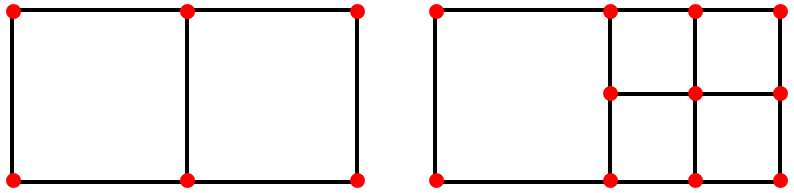
\includegraphics[width=0.85\textwidth]{figures/sec_Intro/locally_refined_vertices.png}
\caption{Local mesh refinement of an initial quadrilateral cell (left) leads to a degenerate pentagonal cell (right) without the use of a hanging node.}
\label{fig::Intro_locally_refined_vertices}
\end{figure}

\noindent This means that, besides being able to accurately model complicated geometries, polytope meshes have benefits that are amenable to future HPC architectures. Specifically, they can reduce cell counts while maintaining equivalent accuracy. Furthermore, they allow for more general cells on non-conforming grids that can arise from either parallel mesh generation or local refinement procedures.

Higher-order FEM basis functions provide a two-fold benefit when used in conjunction with HPCs. First, they provide a richer interpolatory space for the FEM basis functions resulting in increased convergence rates for the discretized solution \cite{ern2013theory}. Second, they can maximize the parallel efficiency on these proposed exascale machines. Low-order spatial discretizations of the DGFEM transport equation may require more mesh cells in the computational domain compared to the number of mesh cells of high-order spatial discretizations. For the DGFEM $S_N$ method, this equates to a greater number of independent linear solves for the low-order discretizations. Since the current and future computational bottlenecks for neutron transport are memory-access related, then higher-order FEM basis functions will be more computationally efficient. This is because the higher-order basis functions can perform more on-process work before memory-access routines are needed.

DSA schemes have been an integral component for solving the DGFEM transport equation for highly diffusive problems. These diffusive neutron problems can consist of energy groups with high within-group scattering ratios and problems with sufficient thermal neutron upscattering and minimal thermal absorption. Many schemes have been proposed over the years to properly discretize the diffusion operator to be consistent with the discretization of the transport equation. In this work, we seek to study a DSA scheme that is compatible with arbitrary polytope meshes and amenable to massively-parallel computations.

In this work, we will answer three specific open questions regarding solutions of the DGFEM $S_N$ transport equations:

\begin{enumerate}
\item Can higher-order 2D polygonal basis functions be used to solve the DGFEM transport equation?
\item Can an efficient and robust DSA scheme be used on arbitrary grids while maintaining scalability to high process counts?
\item Can a parallelizable variant of the Two-Grid acceleration method be derived to accelerate problems dominated by thermal neutron upscattering?
\end{enumerate}

\noindent The methodology, implementation, and results pertaining to these three items are provided in Chapters \ref{sec::BF} and \ref{sec::DSA}.

%%%%%%%%%%%%%%%%%%%%%%%%%%%%%%%%%%%%%%%%%%%%%%%%%%%
%%%   Section - Current State of the Problem
\section{Current State of the Problem}
\label{sec::Intro_Past}

We now provide a brief overview of what consititutes the state-of-the-art in the different topical areas related to this dissertation work. First, we give background information on the Multigroup DGFEM $S_N$ transport equation in Section \ref{sec::Intro_Past_DGFEMMGSn}. Then, we provide a brief explanation of the necessity of DSA schemes in Section \ref{sec::Intro_Past_DSA}. Finally, we detail how the polytope meshes in this work will be generated in Section \ref{sec::Intro_Past_Polytopes}.

%%%%%%%%%%%%%%%%%%%%%%%%%%%%%%%%%%%%%%%%%%%%%%%%%%%
%%%   SubSection - DGFEM Sn Transport
\subsection{Background on the Multigroup DGFEM $S_N$ Transport Equation}
\label{sec::Intro_Past_DGFEMMGSn}

The neutral particle transport equation has a high-dimensional phase space, consisting of 3 spatial variables, 1 energy variable, and 2 angular variables. Many different methodologies have been developed over the years to efficiently discretize and solve each of these variables. We now briefly detail the discretization methods that will be utilized in this work.

For the energy variable, we will utilize the multigroup method since it is the only widely-used energy discretization scheme in deterministic transport \cite{duderstadt1976nuclear,bell1979nuclear}. With the multigroup approximation, the energy domain is broken up into intervals (groups) and then averaged over these intervals with an approximation of the spectral transport solution as the weighting spectrum. This process requires a combination of highly accurate nuclear data libraries such as the Evaluated Nuclear Data File (ENDF) \cite{chadwick2006endf,chadwick2011endf}, the Japanese Evaluated Nuclear Data Library (JENDL) \cite{shibata2002japanese}, and the Joint Evaluated Fission and Fusion Project (JEFF) \cite{koning2006jeff}, as well as high-fidelity processing software such as NJOY \cite{macfarlane2002njoy,kahler2012njoy}, AMPX \cite{dunn2002ampx}, and SCALE \cite{bucholz1982scale} to form the multigroup cross sections. Work is continuously being performed to quantify uncertainties in these cross sections and their effects to solution accuracy \cite{aliberti2006nuclear,jessee2008cross}.

For the angle variable in the transport equation, there are multiple discretization methods we could employ. For this work, we choose to use the discrete ordinates ($S_N$) scheme \cite{carlson1968computing,lewis1984computational}. The $S_N$ method is a collocation discretization scheme where the transport equation is solved along predetermined directions of an angular quadrature set. This method differs strongly from modal expansion schemes such as the $P_N$ or Simplified $P_N$ ($SP_N$) methods \cite{bell1979nuclear,gelbard1960application}. $S_N$ methods are widely used for a variety of applications, but they can suffer from ray effects arising from streaming paths in a heterogeneous problem \cite{lathrop1968ray}. First-collision source approaches are currently used to mitigate these ray effects \cite{lathrop1971remedies,morel_rayeffects}.

This just leaves the choice for spatial discretization remaining. There have been many spatial schemes for the transport equation that we will not consider for this work, including finite difference/volume methods, characteristic methods, collision probability methods, and nodal methods \cite{bell1979nuclear,morel1999self,askew1972characteristics,alcouffe1981review,sanchez1982review}. Instead we choose to employ the DGFEM discretization for our transport problems \cite{reed1973triangularmesh,lesaint1974finite}. The method was originally derived for neutral particle transport problems in the early 1970's. It was immediately employed to solve the transport equation on triangular meshes in the TRIPLET \cite{reed1973triplet} and TRIDENT \cite{seed1977trident,seed1978trident} codes. TRIPLET utilized approximations with various polynomial orders, but TRIDENT was restricted to only linear DGFEM. Subsequent works in 3D have been largely restricted to linear DGFEM approximations on tetrahedral and hexahedral mesh cells \cite{wareing2001discontinuous,morel2005s}. For the most part, only linear basis functions have been used with the DGFEM transport equation as the researchers wanted to focus on accuracy in the thick diffusive limit and the robustness of the spatial discretization. Recently, the works of Wang and Ragusa have analyzed the convergence rates of the DGFEM $S_N$ equations on unstructured triangular meshes with higher-order basis functions \cite{wang2009convergence,wang2009high}.

Traditionally, the DGFEM $S_N$ transport equation has been solved on simplical (triangles and tetrahedra) or tensor-based meshes (quadrilaterals and hexahedra) using linear basis functions. Very recently, there have been advances made to solve these equations on polygonal and polyhedral grids \cite{davidson2008finite,ref::PWLD_stone_adams,ref::PWLD_stone_adams_unstructured,bailey2008phd}. However, this has been relegated to only linear basis functions since the use of polytope finite elements is still in its infancy. Within the past 10 years, the applied mathematics communities have made great strides in the fields of interpolatory functions on arbitrary polytopes \cite{sukumar2006recent}. Even more recently, work has begun on higher-order interpolation schemes \cite{rand2013interpolation}. This means that the capacity to use higher-order basis functions for the DGFEM $S_N$ transport equation on polytope meshes is now realizable. 

%%%%%%%%%%%%%%%%%%%%%%%%%%%%%%%%%%%%%%%%%%%%%%%%%%%
%%%   SubSection - DSA
\subsection{Diffusion Synthetic Acceleration}
\label{sec::Intro_Past_DSA}

For transport calculations involving highly-diffusive media, Diffusion Synthetic Acceleration (DSA) becomes an effective scheme to precondition the DGFEM transport iterations. For these optically thick problems, the traditional Richardson or Source Iteration (SI) schemes become ineffective and prohibitively slow convergence arises \cite{ref::adams_larsen_iter_methods}. There are many different synthetic acceleration schemes that have been proposed over the years, but DSA is the most popular and common method for highly-diffusive problems.

Unfortunately, a continuous finite element (CFEM) discretization of the standard reaction-diffusion equation (the simplest option) is ineffective. This is because we are not guaranteed stability when it is used in conjunction with the DGFEM transport equation on multi-dimensional, unstructured meshes. It was realized that the discretization of the diffusion equations needed to be consistently derived from the discretized transport equation \cite{alcouffe1976stable,alcouffe1977DSA,larsen1982unconditionally_I,larsen1982unconditionally_II,warsa2002fully}. Unfortunately, for higher spatial dimensions, this ``fully-consistent'' DSA scheme constituted a hybrid DGFEM form of the $P_1$ equations that is computationally expensive to solve. Therefore, much work has been performed to develop ``partially-consistent'' DSA schemes that are stable and robust for many mesh types \cite{ref::dsa_DFEM_adams_martin,wareing1991diffusion,ref::DSA_wang_ragusa}. To date, the Modified Interior Penalty (MIP) DSA scheme is the only one that has been shown to be unconditionally stable and effective on unstructured meshes while still being computationally efficient \cite{ref::DSA_wang_ragusa,turcksin2014discontinuous}.

%%%%%%%%%%%%%%%%%%%%%%%%%%%%%%%%%%%%%%%%%%%%%%%%%%%
%%%   SubSection - Polytope Grids
\subsection{Polytope Grid Generation}
\label{sec::Intro_Past_Polytopes}

Since this dissertation work deals with the solution of the transport equation on polytope meshes, we next describe how these grids can be generated. First, we give a brief discussion on the use of bounded Voronoi diagrams to generate polytope meshes. For this work, we will focus on using Voronoi diagrams to form 2D polygonal meshes. Then, these polygonal meshes can be extruded to form 3D polyhedral meshes with prismatic cells. Finally, we give a brief overview on the use of spatial Adaptive Mesh Refinement (AMR) for the DGFEM $S_N$ transport equation. Instead of using hanging nodes, the refined mesh cells will simply form degenerate polytopes.

%%%%%%%%%%%%%%%%%%%%%%%%%%%%%%%%%%%%%%%%%%%%%%%%%%%
%%%   SubSubSection - Voronoi
\subsubsection{Voronoi Mesh Generation}
\label{sec::Intro_Past_Polytopes_Voronoi}

Traditionally, 2D and 3D FEM calculations have been performed on simplical (triangles and tetrahedra) and tensor-based meshes (quadrilaterals and hexahedra), respectively. In fact, it is still a standard practice to refer to any type of mesh as a {\em triangulation} in some communities \cite{ern2013theory}. Many different mesh generation software have been developed to build these simple grids \cite{shewchuk1996triangle,shewchuk2002delaunay,si2015tetgen,geuzaine2009gmsh}. However, multiple fields including {\em computational fluid dynamics} (CFD) and {\em solid mechanics} are now finding benefits in utilizing polytope meshes for their calculations \cite{ref::star_CCM,yip2005automated}.

However, polytope mesh generation is still in its infancy \cite{yip2005automated,sieger2010optimizing,ebeida2011uniform}. In general, polytope meshes have infinite variety in their topological shape and closed-form solutions are impossible. Therefore, polytope mesh generation is defined as a minimization of an energy residual. This is typically performed with Voronoi tesselation (diagram), where the iterative scheme employed is Lloyd's algorithm \cite{lloyd1982least,linde1980algorithm}. There are two main classes of Voronoi mesh generation. The first is based on uniform random sampling known as Maximal Poisson-Disk Sampling (MPS) \cite{ebeida2011uniform,ebeida2011efficient,ebeida2012simple}. MPS inserts Voronoi seed points into the domain without bias and is known as dart-throwing in computer graphics. The second class of Voronoi mesh generation is known as Centroidal Voronoi Tessellation (CVT) \cite{du1999centroidal,valette2004approximated}. CVT is a Voronoi meshing methodology where the seed points are the centroids of the Voronoi regions. These Voronoi regions correspond to the elements (cells) in the resulting polytope mesh. A lightweight CVT algorithm written in MATLAB and based on Lloyd's algorithm is given in \cite{talischi2012polymesher}.

%%%%%%%%%%%%%%%%%%%%%%%%%%%%%%%%%%%%%%%%%%%%%%%%%%%
%%%   SubSubSection - AMR
\subsubsection{Adaptive Mesh Refinement (AMR) for the DGFEM $S_N$ Transport Equation}
\label{sec::Intro_Past_Polytopes_AMR}

As mentioned previously, an alternative method to generating polytope meshes is through the use of spatial Adaptive Mesh Refinement (AMR). Spatial AMR calculations can result in the generation of an irregular mesh (one with hanging nodes) at any refinement level \cite{carey1997computational,plewa2005adaptive}. Looking at the right image in Figure \ref{fig::Intro_locally_refined_vertices}, the colinear vertex along the right face of the unrefined quadrilateral is an example of a hanging node. To the unrefined quadrilateral, this hanging node is not a degree of freedom. However, careful integration must be performed along the face so that the across-face connectivity is preserved for the refined cells. This leads to additional implementation overhead to properly account for the irregular mesh. If we instead use polytope mesh cells, then the unrefined quadrilateral cell with a hanging node can instead be viewed as a degenerate pentagon with two colinear faces. This can ease the implementation burden of AMR methods.

AMR methods have become commonplace across many scientific and engineering fields \cite{plewa2005adaptive,carey1997computational,ramm2003error,karniadakis2013spectral,schwab1998p,solin2003higher}, but are still in their infancy in their use with the DGFEM transport equation \cite{fuhrer1997posteriori,hartmann2002adaptive,dedner2002adaptive,hartmann2003adaptive,ragusa2010two,wang2011standard}. There are three key factors that are required to yield efficient and successful AMR results:

\begin{enumerate}
\item The number of unknowns from the mesh adaptation compared to those resulting from uniform refinement is orders of magnitude smaller while still attaining similar order of accuracy.
\item The meshes resulting from the iterative refinement strategy are close to ``optimal'' and are represented hierarchically as a nest.
\item An efficient {\em a posteriori} method can be used to accurately determine the relative error distribution of a numerical solution on a mesh.
\end{enumerate}

%%%%%%%%%%%%%%%%%%%%%%%%%%%%%%%%%%%%%%%%%%%%%%%%%%%
%%%   Section - Organization
\section{Organization of the Dissertation}
\label{sec::Intro_Organization}

In this introductory chapter, we have presented a summary of work performed. We also gave our motivation for choosing this work as well as a brief discussion of previous work that has directly influenced this dissertation. We conclude this intoduction by briefly describing the remaining chapters of this dissertation.

In Chapter \ref{sec::Sn}, we present the DGFEM formulation for the multigroup, $S_N$ transport equation. We then describe the transport equation's discretization in energy, angle, and space. We have left the FEM spatial interpolation function as arbitrary at this point to be defined in detail in Chapter \ref{sec::BF}. For the spatial variable, we provide the theoretical convergence properties of the DGFEM form. We also detail the elementary assembly procedures to form the full set of spatial equations. We conclude by providing the methodology to be used to solve the full phase-space of the transport problem.

In Chapter \ref{sec::BF}, we present all the finite element basis functions that we will use in this work. In two dimensions, we present four different linearly-complete polygonal coordinate systems that we will use to generate our finite element basis functions. We then present the methodology that converts each of these linear coordinate systems into quadratically-complete coordinates for use as higher-order basis functions. We also present the single linearly-complete polyhedral coordinate system that we will use for the 3D transport problems.

In Chapter \ref{sec::DSA}, we present the methodologies to be used for DSA preconditioning of the DGFEM transport equation for optically thick problems. We give a discontinuous form of the diffusion equation which can be used on 2D and 3D polytope grids. The theoretical limits of the DSA scheme are analyzed, and we conclude with a real-world problem of accelerating the thermal neutron upscattering of a large multigroup, heterogeneous transport problem. In doing so, we demonstrate that our methodology will work on massively-parallel computer architectures.

We then finalize this dissertation work by drawing conclusions and discussing open topics of research stemming from this dissertation in Chapter \ref{sec::Conclusions}. We note that our detailed literature reviews, numerical results, and conclusions pertaining to each topic are presented in their corresponding chapters.

Additional material that is not included in the main body of the dissertation for the sake of brevity is appended for completeness. The appendices are organized in a simple manner:

\begin{itemize}
\item Appendix \ref{sec::appendix_SN}: addendum to Section \ref{sec::Sn}, corresponding to additional material relating to the multigroup $S_N$ equations.
\item Appendix \ref{sec::appendix_BF}: addendum to Section \ref{sec::BF}, corresponding to additional material relating to the various polytope coordinate systems to be utilized as finite element basis functions.
\item Appendix \ref{sec::appendix_DSA}: addendum to Section \ref{sec::DSA}, corresponding to additional material relating to DSA preconditioning on polytope grids.
\end{itemize}